\chapter{Apache Kafka}
\label{intro-kafka}

As this thesis is about the implementation of a message broker that correlates
to the functionalities Apache Kafka provide, we describe in the following the
components and functionalities of Apache Kafka in the current state (Version
0.8.2). This shall provide a basis for further comparison (see \ref{survey-broker}) with
more traditional broker systems, which is why won't provide any implementation
specific details in this section but describe the concepts in a higher level of
abstractness instead. Thus, it is also an overview and the initial position of our
own implementation (see \todo{ref}), in which Chapter the implementation
specific aspects will be resolved in detail. 

\section{Background}

Apache Kafka was initially developed at LinkedIn\cite{linkedin} and subsequently
released as an open source project with the Apache Software
Foundation\cite{apachefoundation}. 
\\ \\
Initially at LinkedIn the landscape was overwhelmed by the complexity due to
point-to-point (\ref{intro-messaging-pointtopoint})
pipelines that delivered data to a single destination with no
integration between. Messages were written to aggregated files and then copied
to ETL servers and further loaded into data warehousing and batch
processing (\ref{intro-datastream-batchprocessing})
clusters. Thus, this service included the lack of real-time data access which
is---especially for a data driven company that populates activity-driven news
feeds---an essential requirement. In fact, this fragility and complexity of this
pipeline lead to inevitable delays in adding new types of activity data.
Besides the feature wise limitations, also the detection time of operational
problems increased over time due to the ever-increasing pressure on the latency
of the data warehouse ETL processes. This could have been solved solved with
stream processing systems (\ref{intro-datastream-streamprocessing}) but again, 
due to the lack of any central platform (\ref{intro-datastream-centralplatform})
that can provide continuous data, was not supported at this point.
\\ \\
First attempts towards a piece of infrastructure (e.g. broker) that can server
stream and batch processing systems were made by experimenting with
ActiveMQ\cite{activemq}. During tests under full production load they ran into
several significant problems. It turned out that if the queue backed up beyond what could
be kept in memory, performance would severely degrade due to heavy amounts of
random I/O. Inefficiencies had to be accepted regarding clustered consumers
requiring duplicating the data for each consumer in a separate queue. Further
difficulties were faced with ActiveMQ's built in persistence mechanism that lead
to very long restart times. 
\todo[inline]{well, reasons are not that overwhelming honestly...}
According to LinkedIn it would have been possible to provide enough buffer to
keep the ActiveMQ brokers above water but would have required hundred servers to
process a subset of activity data. As a result, the decision was made to build a
custom piece of messaging infrastructure targeting high-volume scale-out
deployment and thus serve batch and stream processing systems. 


\section{Characteristics}
- Zitat: One key feature of Kafka is its functional simplicity. While there is a
lot of sophisticated engineering under the covers, Kafka’s general functionality
is relatively straightforward. Part of this simplicity comes from its
independence from any other applications (excepting Apache ZooKeeper)

\section{Use Cases}
\begin{description}
    \item [Traditional message broker]
    \item [Log aggregation]
    \item [Stream processing] Kafka's strong durability is very useful in the
        context of stream processing
\end{description}

\section{The Log}
Apache Kafka uses a so-called commit log for managing messages within the
broker. This log has nothing in common with "application logging", as traces of
a software designed for human read. Instead, logs in the context of distributed systems
are designed for programmatic access. Basically it is a simple, append-only data
structure which contains a sequence of records ordered by time whereas each
entry is assigned to an unique number, called offset. Thanks to the strict
ordering insight a log the record offset can be used as timestamp whereas a log
gets decoupled from any time system.

\begin{figure}[H]
    \centering
    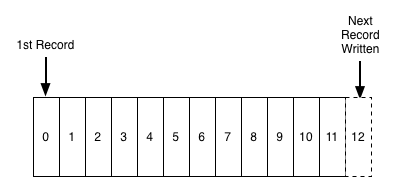
\includegraphics[width=0.4\textwidth]{images/log.png}
    \caption{The  Log}
    \label{fig:the-log}
\end{figure}

Apache Kafka handles a own log for every
topic whereas the log handles all published messages as single records. For
improving throughput and fault tolerance, Kafka can partition a Log

\begin{figure}[H]
    \centering
    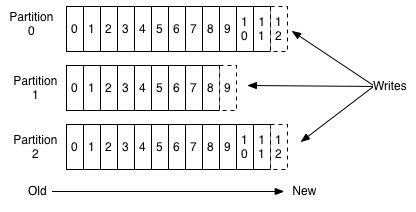
\includegraphics[width=0.5\textwidth]{images/log_anatomy.png}
    \caption{Partitioned Log}
    \label{fig:the-log}
\end{figure}

Logs originally come from databases where they are used to for replication
whereas the log includes records of what happened. Describing every replica by
the maximum log entry it has processed, the problem of coordinating
states of getting replicas is getting much easier. Apache Kafka uses this
approach for consumption of messages. Every consumer knows its actual offset and
advance it linearly as it reads messages from the log. The log can be seen as a
re-playable record of history whereas a consumer also can reset to an older
offset to reprocess.

\begin{figure}[H]
    \centering
    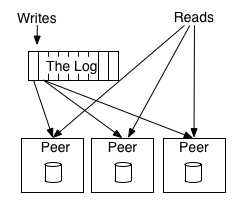
\includegraphics[width=0.4\textwidth]{images/state-machine-replication.png}
    \caption{Log used for replication}
    \label{fig:the-log}
\end{figure}

\section{Components}
\subsection{Persistance}
- disk are fast with linear writes -> example: 7200rpm raid5 ~600MB/s
- operating system read/write ahead
- keep page cache staying warm and store compact byte structure rather than individual objects
- maintaining coherency between the cache and filesystem in the OS
- All data is immediately written to a persistent log on the filesystem without necessarily flushing to disk. In effect this just means that it is transferred into the kernel's pagecache.see also: https://www.varnish-cache.org/trac/wiki/ArchitectNotes
- Instead of  a per-consumer queue with an associated BTree or other general-purpose random access data structures
  a persistent queue could be built on simple reads and appends to files
  This structure has the advantage that all operations are O(1) and reads do not block writes or each other.
- performance is completely decoupled from the data size
- unlimited disk space without any performance penalty means that we can provide some features like retain messages for a relative long period (say a week)

- for each topic a folder
- separate folders over partitions (1;2) -> topic\_0; topic\_1
- file name: offset of the first message it contains (next file: S bytes (max log size, given in configuration) from previous file)
- file format: sequence of log entries
- log entry: N (4 byte integer -> message length) followed by message (N message bytes)
- message: unique identifier (64 bit integer offset -> byte position of the start of this message in the stream of all messages ever sent to that topic on that partition)

On-disk format of a message:

offset: 8 bytes
message length : 4 bytes (value: 1+4+n) 
magic value  : 1 byte
crc            : 4 bytes
payload        : n bytes
    ?:              : 1 byte
    ?:              : 4 bytes
    message length  : 4 bytes
    message         : n bytes

\subsection{Message Delivery}

\subsection{Replication}

\subsection{Compression}

\subsection{Batching}

\subsection{The Producer}

\subsection{The Consumer}
While many brokered message queue systems have the broker maintain the state of
its consumers, Kafka does not.

\subsubsection{Grouping}

\subsubsection{Ordering (offset)}

\section{Configuration Management (Zookeeper)}
\subsection{PAXO Algorithm}
